% GNUPLOT: LaTeX picture with Postscript
\begingroup
  \makeatletter
  \providecommand\color[2][]{%
    \GenericError{(gnuplot) \space\space\space\@spaces}{%
      Package color not loaded in conjunction with
      terminal option `colourtext'%
    }{See the gnuplot documentation for explanation.%
    }{Either use 'blacktext' in gnuplot or load the package
      color.sty in LaTeX.}%
    \renewcommand\color[2][]{}%
  }%
  \providecommand\includegraphics[2][]{%
    \GenericError{(gnuplot) \space\space\space\@spaces}{%
      Package graphicx or graphics not loaded%
    }{See the gnuplot documentation for explanation.%
    }{The gnuplot epslatex terminal needs graphicx.sty or graphics.sty.}%
    \renewcommand\includegraphics[2][]{}%
  }%
  \providecommand\rotatebox[2]{#2}%
  \@ifundefined{ifGPcolor}{%
    \newif\ifGPcolor
    \GPcolortrue
  }{}%
  \@ifundefined{ifGPblacktext}{%
    \newif\ifGPblacktext
    \GPblacktextfalse
  }{}%
  % define a \g@addto@macro without @ in the name:
  \let\gplgaddtomacro\g@addto@macro
  % define empty templates for all commands taking text:
  \gdef\gplbacktext{}%
  \gdef\gplfronttext{}%
  \makeatother
  \ifGPblacktext
    % no textcolor at all
    \def\colorrgb#1{}%
    \def\colorgray#1{}%
  \else
    % gray or color?
    \ifGPcolor
      \def\colorrgb#1{\color[rgb]{#1}}%
      \def\colorgray#1{\color[gray]{#1}}%
      \expandafter\def\csname LTw\endcsname{\color{white}}%
      \expandafter\def\csname LTb\endcsname{\color{black}}%
      \expandafter\def\csname LTa\endcsname{\color{black}}%
      \expandafter\def\csname LT0\endcsname{\color[rgb]{1,0,0}}%
      \expandafter\def\csname LT1\endcsname{\color[rgb]{0,1,0}}%
      \expandafter\def\csname LT2\endcsname{\color[rgb]{0,0,1}}%
      \expandafter\def\csname LT3\endcsname{\color[rgb]{1,0,1}}%
      \expandafter\def\csname LT4\endcsname{\color[rgb]{0,1,1}}%
      \expandafter\def\csname LT5\endcsname{\color[rgb]{1,1,0}}%
      \expandafter\def\csname LT6\endcsname{\color[rgb]{0,0,0}}%
      \expandafter\def\csname LT7\endcsname{\color[rgb]{1,0.3,0}}%
      \expandafter\def\csname LT8\endcsname{\color[rgb]{0.5,0.5,0.5}}%
    \else
      % gray
      \def\colorrgb#1{\color{black}}%
      \def\colorgray#1{\color[gray]{#1}}%
      \expandafter\def\csname LTw\endcsname{\color{white}}%
      \expandafter\def\csname LTb\endcsname{\color{black}}%
      \expandafter\def\csname LTa\endcsname{\color{black}}%
      \expandafter\def\csname LT0\endcsname{\color{black}}%
      \expandafter\def\csname LT1\endcsname{\color{black}}%
      \expandafter\def\csname LT2\endcsname{\color{black}}%
      \expandafter\def\csname LT3\endcsname{\color{black}}%
      \expandafter\def\csname LT4\endcsname{\color{black}}%
      \expandafter\def\csname LT5\endcsname{\color{black}}%
      \expandafter\def\csname LT6\endcsname{\color{black}}%
      \expandafter\def\csname LT7\endcsname{\color{black}}%
      \expandafter\def\csname LT8\endcsname{\color{black}}%
    \fi
  \fi
    \setlength{\unitlength}{0.0500bp}%
    \ifx\gptboxheight\undefined%
      \newlength{\gptboxheight}%
      \newlength{\gptboxwidth}%
      \newsavebox{\gptboxtext}%
    \fi%
    \setlength{\fboxrule}{0.5pt}%
    \setlength{\fboxsep}{1pt}%
    \definecolor{tbcol}{rgb}{1,1,1}%
\begin{picture}(8640.00,5760.00)%
    \gplgaddtomacro\gplbacktext{%
      \csname LTb\endcsname%%
      \put(814,704){\makebox(0,0)[r]{\strut{}$0$}}%
      \put(814,1478){\makebox(0,0)[r]{\strut{}$20$}}%
      \put(814,2251){\makebox(0,0)[r]{\strut{}$40$}}%
      \put(814,3025){\makebox(0,0)[r]{\strut{}$60$}}%
      \put(814,3798){\makebox(0,0)[r]{\strut{}$80$}}%
      \put(814,4572){\makebox(0,0)[r]{\strut{}$100$}}%
      \put(814,5346){\makebox(0,0)[r]{\strut{}$120$}}%
      \put(946,484){\makebox(0,0){\strut{}$0$}}%
      \put(2215,484){\makebox(0,0){\strut{}$2$}}%
      \put(3484,484){\makebox(0,0){\strut{}$4$}}%
      \put(4753,484){\makebox(0,0){\strut{}$6$}}%
      \put(6022,484){\makebox(0,0){\strut{}$8$}}%
      \put(7291,484){\makebox(0,0){\strut{}$10$}}%
    }%
    \gplgaddtomacro\gplfronttext{%
      \csname LTb\endcsname%%
      \put(2009,5181){\makebox(0,0)[l]{\strut{}Upper Bound}}%
      \csname LTb\endcsname%%
      \put(2009,4851){\makebox(0,0)[l]{\strut{}$(\mathbf{C}+\mathbf{T})_2$ - Bocharov et al.}}%
      \csname LTb\endcsname%%
      \put(2009,4521){\makebox(0,0)[l]{\strut{}$(\mathbf{C}+\mathbf{R})_3^H$ - Gustafson et al.}}%
      \csname LTb\endcsname%%
      \put(2009,4191){\makebox(0,0)[l]{\strut{}$(\mathbf{C}+\mathbf{R})_3^E$ - Gustafson et al.}}%
      \csname LTb\endcsname%%
      \put(2009,3861){\makebox(0,0)[l]{\strut{}$(\mathbf{C}+\mathbf{D})_3^H$ - This work}}%
      \csname LTb\endcsname%%
      \put(209,3121){\rotatebox{-270.00}{\makebox(0,0){\strut{}$N_{\mathcal{G}}$}}}%
      \put(4594,154){\makebox(0,0){\strut{}$\log_{10}(\epsilon^{-1})$}}%
      \colorrgb{0.90,0.62,0.00}%%
      \put(7577,4406){\rotatebox{37.00}{\makebox(0,0){\scriptsize $3\log_{2}(1/\epsilon)-5.65$}}}%
      \colorrgb{0.00,0.62,0.45}%%
      \put(7133,4379){\rotatebox{37.00}{\makebox(0,0){\scriptsize $4.9\log_{3}(1/\epsilon)-2.16$}}}%
    }%
    \gplbacktext
    \put(0,0){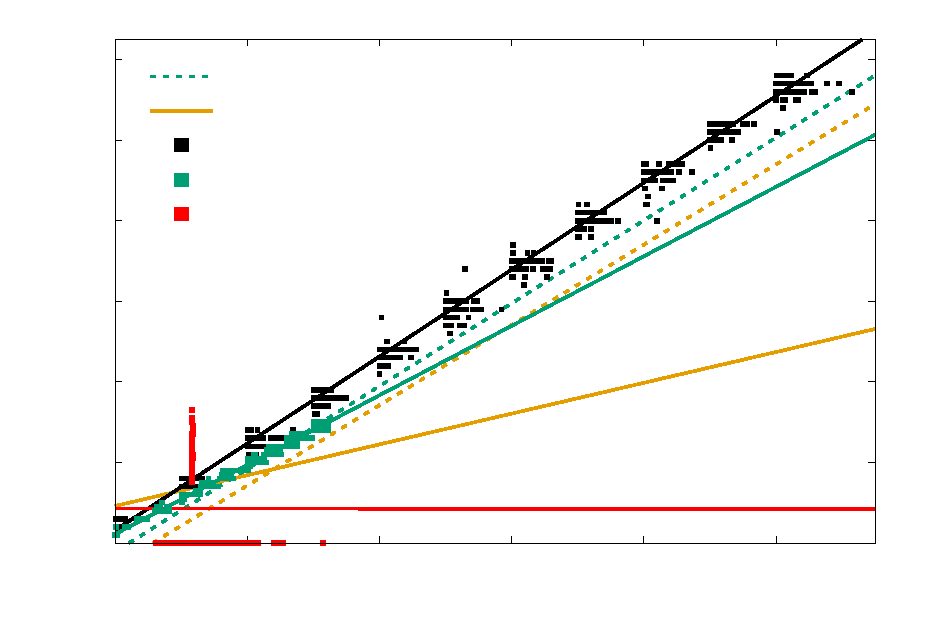
\includegraphics[width={432.00bp},height={288.00bp}]{tve_gnu}}%
    \gplfronttext
  \end{picture}%
\endgroup
